\documentclass[12pt]{article}

% ----------------------------------------------------------------------
% Definir packages externos, língua, margens, tipos de letra, novos 
% comandos e cores
% ----------------------------------------------------------------------
\usepackage[utf8]{inputenc} % Codificação utilizada
\usepackage[english]{babel} % Idioma de escrita

\usepackage[export]{adjustbox} % Alinhar imagens
\usepackage{amsmath} % Comandos extra para escrita matemática
\usepackage{amssymb} % Símbolos matemáticos
\usepackage{anysize} % Personalizar as margens
    \marginsize{2cm}{2cm}{2cm}{2cm} % {esquerda}{direita}{cima}{baixo}
\usepackage{appendix} % Apêndices
\usepackage{cancel} % Cancelar expressões
\usepackage{caption} % Legendas
    \DeclareCaptionFont{newfont}{\fontfamily{cmss}\selectfont}
    \captionsetup{labelfont={bf, newfont}}
%\usepackage{cite} % Citações, tipo [1 - 3]
\usepackage{color} % Colorir texto
\usepackage{fancyhdr} % Cabeçalho e rodapé
    \pagestyle{fancy}
    \fancyhf{}
    \fancyhead[L]{\footnotesize\fontfamily{cmss}\selectfont IST} % Esquerda do cabeçalho
    \fancyhead[R]{\footnotesize\fontfamily{cmss}\selectfont ULisboa} % Direita do cabeçalho
    \fancyfoot[L]{\footnotesize\fontfamily{cmss}\selectfont Projeto de Sistemas Digitais} % Esquerda do rodapé
    \fancyfoot[C]{\thepage} % Centro do rodapé
    \fancyfoot[R]{\footnotesize\fontfamily{cmss}\selectfont LEEC} % Direita do rodapé
    \renewcommand{\footrulewidth}{0.4pt} % Régua do rodapé
\usepackage{float} % Utilizar o especificador [H] nas figuras
\usepackage{graphicx} % Imagens em LaTeX
\usepackage[colorlinks = true, plainpages = true, linkcolor = istblue, urlcolor = istblue, citecolor = istblue, anchorcolor = istblue]{hyperref}
\usepackage{csquotes}
\usepackage{listings}
\usepackage{amsmath}
\usepackage{indentfirst} % Primeiro parágrafo
\usepackage{siunitx} % Unidades SI
\usepackage{subcaption} % Subfiguras
\usepackage{titlesec} % Tipo de letra
    \titleformat{\section}{\fontfamily{cmss}\selectfont\Large\bfseries}{\thesection}{1em}{}
    \titleformat{\subsection}{\fontfamily{cmss}\selectfont\large\bfseries}{\thesubsection}{1em}{}
    \titleformat{\subsubsection}{\fontfamily{cmss}\selectfont\normalsize\bfseries}{\thesubsubsection}{1em}{}
    \fancyfoot[C]{\fontfamily{cmss}\selectfont\thepage}

% Encher de texto aleatório (apagar)
\usepackage{lipsum}
\usepackage{duckuments}
\usepackage[table]{xcolor}

% Novos e renovar comandos
\newcommand{\sen}{\operatorname{\sen}} % Definição da função seno
\newcommand{\HRule}{\rule{\linewidth}{0.5mm}} % Definição de uma régua
\renewcommand{\appendixpagename}{\LARGE \fontfamily{cmss}\selectfont Apêndices}
\renewcommand{\appendixtocname}{Apêndices}

% Cores
\definecolor{istblue}{RGB}{3, 171, 230}
\definecolor{dkgreen}{rgb}{0,0.6,0}
\definecolor{gray}{rgb}{0.5,0.5,0.5}

%importar bibliografia
\usepackage[
backend=biber,
style=alphabetic,
sorting=nyt,
]{biblatex}
\addbibresource{refs.bib} 

%%%%%%%%%%%%%%%%%%%%%%%%%%%%%%%%%%%%%%%%%%%%%%%%%%%%%%%%%%%%%%%%%%%%%%%%
%                               Documento                              %
%%%%%%%%%%%%%%%%%%%%%%%%%%%%%%%%%%%%%%%%%%%%%%%%%%%%%%%%%%%%%%%%%%%%%%%%
\begin{document}

% ----------------------------------------------------------------------
% Capa
% ----------------------------------------------------------------------
\begin{center}
    \begin{figure}
        \vspace{-1.0cm}
        
\includegraphics[scale = 0.3, left]{images/IST_A.eps} % Tipo de assinatura do IST
    \end{figure}
    \mbox{}\\[2.0cm]
    \textsc{\Huge Projeto de Sistemas Digitais}\\[2.5cm]
    \textsc{\LARGE MEEC}\\[2.0cm]
    \HRule\\[0.4cm]
    {\large \bf {\fontfamily{cmss}\selectfont Complex Determinant Computation} [\texttt{EN}]}\\[0.2cm]
    \HRule\\[1.5cm]
\end{center}

\begin{flushleft}
    \textbf{\fontfamily{cmss}\selectfont Authors:}
\end{flushleft}

\begin{center}
    \begin{minipage}{0.4\textwidth}
        \begin{flushleft}
            Alexandre Santos (99884)\\
            Nuno Abreu (103416)\\
            Carlos Reis (103166) \\
        \end{flushleft}
    \end{minipage}%
    \begin{minipage}{0.6\textwidth}
        \begin{flushright}
            \href{mailto:ares.santos@tecnico.ulisboa.pt}{\texttt{ares.santos@tecnico.ulisboa.pt}}\\
            \href{mailto:nuno.g.tribolet.de.abreu@tecnico.ulisboa.pt}{\texttt{nuno.g.tribolet.de.abreu@tecnico.ulisboa.pt}}\\
            \href{mailto:guilherme.garcia@tecnico.ulisboa.pt}{\texttt{guilherme.garcia@tecnico.ulisboa.pt}}\\
            
        \end{flushright}
    \end{minipage}


\end{center}
    
\begin{flushleft}
    \large $\boxed{\text{\bf \fontfamily{cmss}\selectfont Group 10}}$\\[4.0cm]
\end{flushleft}
    
\begin{center}
    \large \bf \fontfamily{cmss}\selectfont 2024/2025 -- 1st Semester, P1
\end{center}

\thispagestyle{empty}

\setcounter{page}{0}

\newpage

% ----------------------------------------------------------------------
% Conteúdo
% ----------------------------------------------------------------------


\section{Introduction}
The following report pertains to the third laboratory task of Project of Digital Systems.

The objective is to design a circuit that computes determinants of complex valued matrices, with VHDL hardware description language and making use of simulation and logic synthesis. The circuit is then implemented with the AMD Vivado™ tool in the Digilent Basys 3™ FPGA board. 

\section{Data-flow Graph}
To start the work a data-flow graph was made accordingly with the operations needed to compute the determinant's. The result is presented in image \ref{fig:dataflow} corresponds to one loop iteration of the algorithm. This graph shows the serialization limitation of the sequence of operations needed and allows us to make a priority list based on the critical path.

\begin{figure}[H]
	\centering
	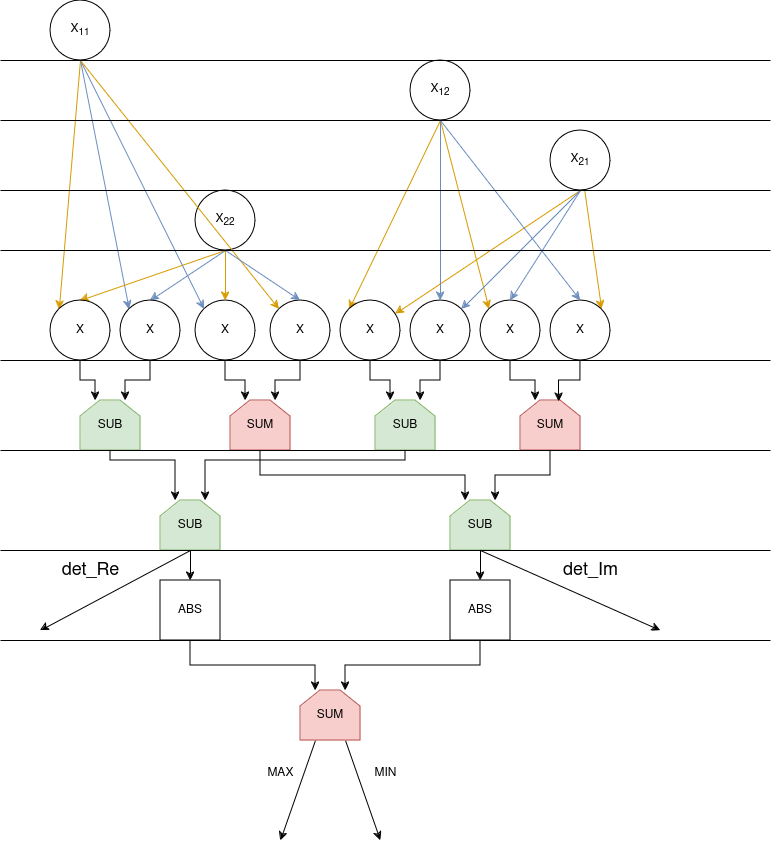
\includegraphics[width=0.55\linewidth]{images/DataFlowGraph.png}
	\caption{Data-Flow Graph}
	\label{fig:dataflow}
\end{figure}




\begin{figure}[H]
	\centering
	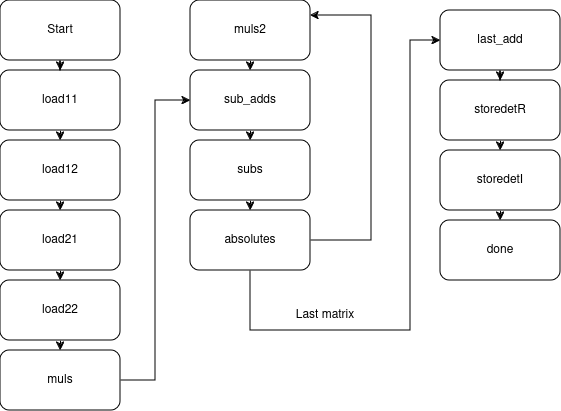
\includegraphics[width=0.55\linewidth]{images/FSM_lab3.png}
	\caption{Finite State Machine}
	\label{fig:fsm}
\end{figure}

\section{Circuit Design}
\subsection{Data-Path}
Utilizing the data-flow graph as a base for our data-path design. We designed the data-path already as a pipeline in order to make the operations faster and efficient. The final design as three main parts, loading from memory, determinants operation and operations done to the determinants, can be seen in the figure \ref{fig:datapath}.

The first part is the registers that contain all values, real and imaginary, of the matrix. This values are loaded from memory and takes four clock cycles because only one value at a time from the matrix can be retrieved. The managing of what loads what for the register is done by the control unit.

The second part is the operations to calculate the determinants, this is done by realizing the operation $$DET=(((R11*R22)-(I11*I22))-((R12*R21)-(I12*I21))) $$. This is done in three stages of the pipeline placing the real and imaginary values of the determinant of the matrix in registers REG\textunderscore DETR and REG\textunderscore DETI. This registers outputs will be then also connected to a multiplexer for the output memory.

The third and last part is responsible to calculate the average and determine the highest and lowest absolute value of the determinant of all matrix calculated. to calculate the average of all eight matrix we use a ALU and register so as each determinant is ready the control unit enables the register and the new determinant is added. In the end when sent to the multiplexer of the output memory the sum is divided by eight. To determine the highest and lowest determinant of the absolute values the last part in the data-path. The absolute operation is done by seeing if the signed bit is positive or negative connects to a multiplexer, if is a 1 the determinant is negated and added 1 this way obtaining the absolute if it is 0 the value of the previous register will just pass. After this the imaginary and real part are just summed and then compared to the previous max and min values saved in registers if they are they are saved. There is also a counter that saves the matrix number that corresponds to the value saved. This then is used to light up the correct leds. 
\begin{figure}[H]
	\centering
	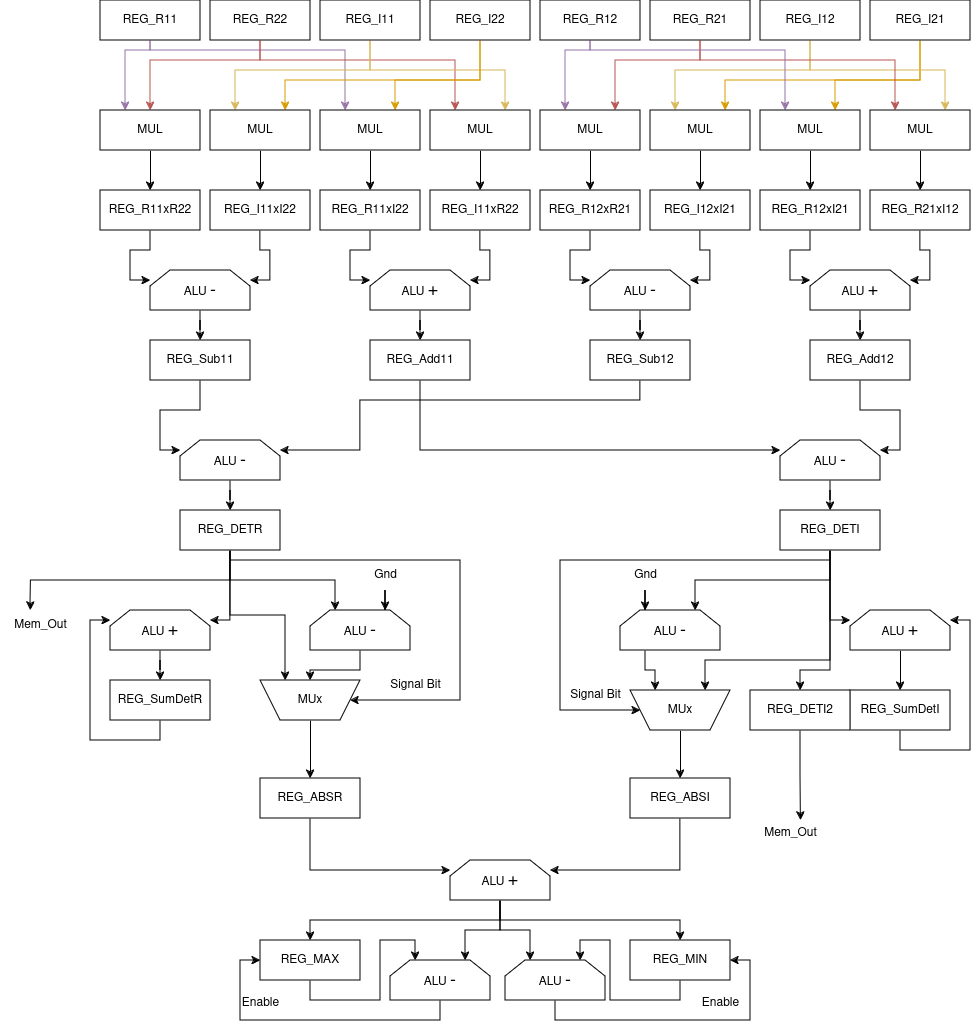
\includegraphics[width=0.75\linewidth]{images/DataPath.png}
	\caption{Data-Flow Graph}
	\label{fig:datapath}
\end{figure}


\subsection{Control Unit}
The control unit implements a finite state machine with 14 states. A start state awaits for the command to begin calculations(BTNR), followed by 5 states to fill up the pipeline, 4 states that repeat until the last matrix arrives at the datapath, 3 states to empty it and one done state where the machine and presents the results.
Two counters keep trace of input and output memory addresses.

Each state takes up one clock cycle, except for the start and done states which extend indefinitely. A reset signal returns the control to the start state, the counters to 0 and all registers to 0.


For simplicity, we will only show the simulations done for MemIn1.

The test-bench used is very simple. All it does is reset the circuit followed by handling the clock.

The clock cycle of the circuit was set to 18ns in the constraints and the same value was used for the test-bench. This left us with a WNS of 3.697ns.


Figure is a portion of the behavioral simulation of the circuit. We can observe the different states and the data out change as the calculations finish and write enable toggles. Notice also how this is address 3 of the memory, the final value of -536804112 is correct.


Figure is a similar cutout, but now from the Post-Implementation Timing Simulation. We now can't see the states, however we can see that the write enable and data out behaviour is the same. Notice how the result of -343976512 is correct for address 2.

\section{Simulations and Results}
This section elaborates on different sets of simulations that were employed to verify the behaviour of our circuit. Various testbenches were developed to check behaviout at different stages of the development process.

For all simulations and fisical tests assume that MemIn is initialized with the values corresponding to the seed 46. Other values where tested and functioned in the same manner.
\subsection{DataPath}
The file datapath\_tb.vhd implements a testbench for the datapath unit of the circuit. 
It first resets the component and afterwards excites the inputs with a known matrix. This allows the developer to observe the latency of the circuit and also verify the answer. It was used extensively for debugging. 

The current matrix used in the test bench is:
\begin{equation*}
	\begin{vmatrix} 2+i & 2+2i \\ 
					1-i & 1+4i 
	\end{vmatrix} 
	= -7 + 10i
\end{equation*}

\begin{figure}[!htp]
	\centering
	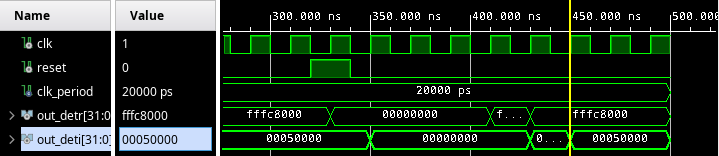
\includegraphics[width=0.5\linewidth]{images/simDataPath.png}
	\caption{Data path simulation}
	\label{fig:simData}
\end{figure}

Notice how in figure \ref{fig:simData} it takes 4 cycles for the real portion of the determinant to be set, and it takes 5 for the imaginary. Calling back to figure \ref{fig:datapath} we can see how that is as expected due to the number of registers.

\subsection{Control Unit}
\subsection{Circuit}
An intermediate testbench was created for the total designed circuit, but without the IO and FPGA integration.
The circuit\_tb.vhd file instantiates said circuit as well as the MemIn component and does the necessary connections.

\begin{figure}[!htp]
	\centering
	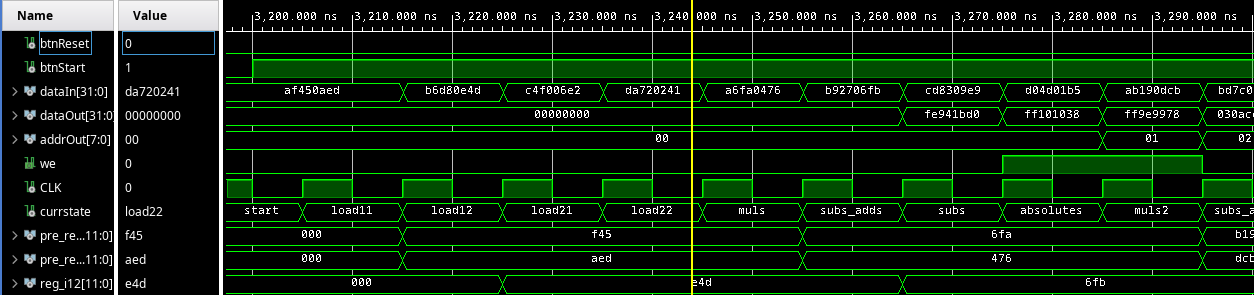
\includegraphics[width=0.7\linewidth]{images/simCircuit.png}
	\caption{Siplified circuit simulation}
	\label{fig:simCircuit}
\end{figure}

Notice how in figure \ref{fig:simCircuit} the first write enable happens after 7 clock cycles. This is due to the memory accesses. It takes 4 clock cycles for all values to be fetched. We can see this in the registers present in the waveform.

The last WE occurs after 38 clock cycles.

\subsection{Top Circuit}
The top circuit was the file provided that handled the IO and connections with the FPGA board. As well as the component file a simulation source was also provided, top\_circuit\_tb.vhd. 
This testbench was used mostly for the demonstration and post implementation simulations. The following is an excerpt from the post implementation timing simulation.


\begin{figure}[!htp]
	\centering
	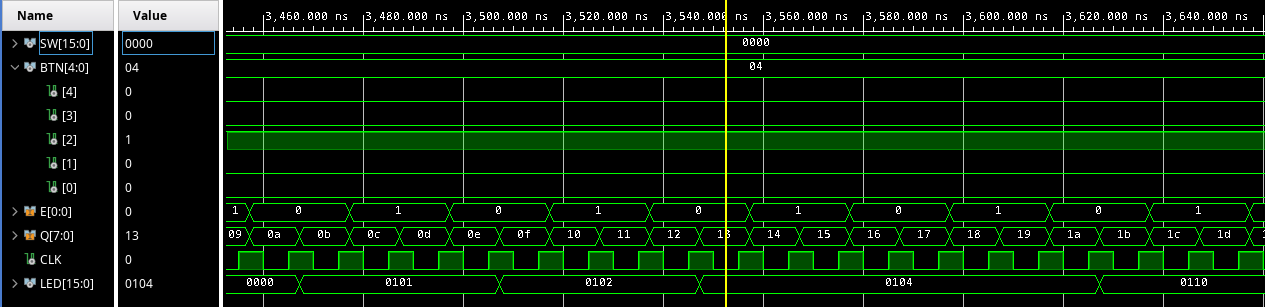
\includegraphics[width=0.7\linewidth]{images/simTopCircuit.png}
	\caption{Top circuit simulation}
	\label{fig:simTopCircuit}
\end{figure}

Notice how the board LEDs are now visible in the simulation. We can see how they update around 2-3 clock cycles after the write enable which is consistent with the schematic in figure \ref{fig:datapath}.
We can also observe how values are set around the midpoint of the high portion of the clock. Possible timing improvements will be discussed later.

\subsection{Fisical Board test}
The fisical board test went as expected.
Serial communication with the board was handled through the cu command (see man cu(1) for sepecifications).

All results were correct and as expected.

\section{Possible improvements}
Besides pipelining, no other timing or throughput improvements were implemented.

The Worst Negative Slack has a value of 3.868ns which implies possible over clocking capabilities. In fact simulations using an 8ns clock cycle yielded cprrect results. However this was not fully implemented nor was it tested on the board.

In the datapath certain pipeline stages could have been joint together due to the fact that they are composed only of simple ALU maths like sums and subtractions. This could have lead to improved throughput and a overall faster circuit.

\section{Conclusion}
Through this laboratory we successfully simulated and implemented a datapath, control unit(with two counters for address tracking) components and memory access.

The focus of this project was to design a circuit in an efficient way to compute various determinants. This was achieved through pipelining.
  
We implemented the final circuit to test if its behaviour was as designed and verified its outputs with the provided script. This allowed us to
find errors in our design, correct them in timely manner and fine tune the clock period to a reasonable value maintaining a positive Worst Negative Slack.

Further optimizations were discussed such as pipelining and reducing the number of registers. Both solutions implied a trade-off, the former requiring more components and the latter increasing the clock period thus decreasing throughput.

\printbibliography
\end{document}

